\section{Additional figures}

\begin{figure}[h]
\centering
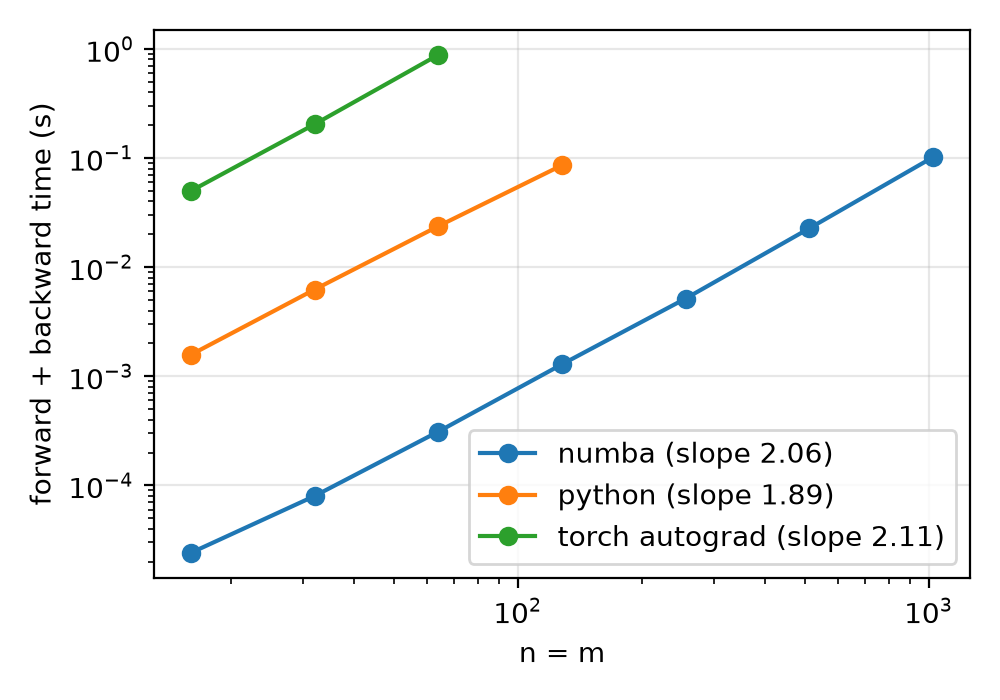
\includegraphics[width=0.55\linewidth]{timing.png}
\caption{Forward + backward time vs.\ length $n=m$ (log-log). All implementations are quadratic; Numba is $\sim$65$\times$ faster than the same code in pure Python and $\sim$2400$\times$ faster than a cell-by-cell PyTorch forward differentiated by autograd ($n=64$).}
\label{fig:timing}
\end{figure}

\todo{qualitative figures: barycenters on ECG200 (paper Fig.~5), interpolation on GunPoint (Fig.~4), $k$-means clusters on CBF (Fig.~6), forecasts on ShapesAll (Fig.~1).}
